%---------------------------------------------------------------------------

\begin{frame}
	\frametitle{Plan prezentacji}

	\begin{enumerate}
		\item Algorytm Scale Space
		\item Standard OpenCL
		\item Wyniki
	\end{enumerate}

\end{frame}

%---------------------------------------------------------------------------

%Jednym z istotniejszych problemów podczas automatycznego przetwarzania i analizy obrazów jest wybór skali.

%Obrazy mogą być rejestrowane w~różnych skalach.

\begin{frame}
	\frametitle{Algorytm Scale Space}
	\begin{block}{Scale Space}
		Algorytm służący do przedstawiania sygnałów w reprezentacji skali.
	\end{block}
	Można go zastosować do dowolnych sygnałów. Praca skupia się na wykorzystaniu algorytmu do przetwarzania obrazów.

\end{frame}

%---------------------------------------------------------------------------
\begin{frame}
	\frametitle{Podstawy matematyczne}
	
	\begin{center}
		$ g(x,y,\sigma)= \frac{1}{2 \cdot \pi \cdot \sigma ^ {2} }\cdot e^{(-\frac{x^{2} + y^{2}}{2 \cdot \sigma ^{2}})} $

	\begin{figure}[h]
		\begin{center}
			\begin{subfigure}[b]{4.5cm}
				\centering
				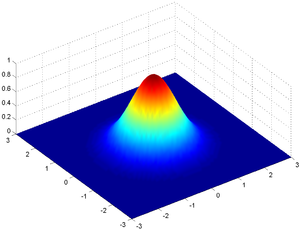
\includegraphics[width=4.5cm]{gaussian2d.png}
			\end{subfigure}
			~
			\begin{subfigure}[b]{4.5cm}
				\centering
				\includegraphics[width=4.5cm]{gaussian2dcoef.png}
			\end{subfigure}
		\end{center}
	\end{figure}
		
	\end{center}
	
	Do wyznaczenia przestrzeni skali stosuje się filtry Gaussa. 
	
	%Poniżej przedstawiono sposób wyznaczania współczynników filtra w przestrzeni dwuwymiarowej.
	
\end{frame}
%---------------------------------------------------------------------------
\begin{frame}
	\frametitle{Algorytm Scale Space dla obrazów}


	\begin{figure}[h]
		\begin{center}
			\begin{subfigure}[b]{3cm}
				\centering
				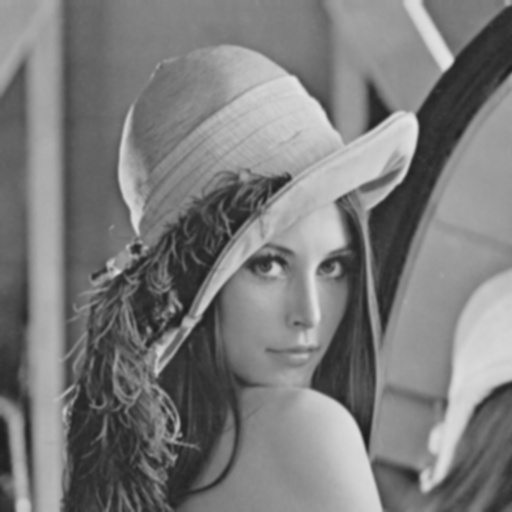
\includegraphics[width=2.5cm]{Lena_scales1.jpg}
				\caption{$\sigma = x$, $N = 3$}
			\end{subfigure}
			~
			\begin{subfigure}[b]{3cm}
				\centering
				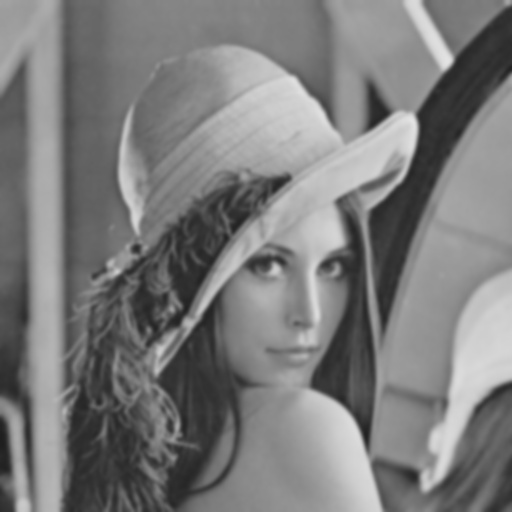
\includegraphics[width=2.5cm]{Lena_scales2.jpg}
				\caption{$\sigma = x$, $N = 5$}
			\end{subfigure}
			~
			\begin{subfigure}[b]{3cm}
				\centering
				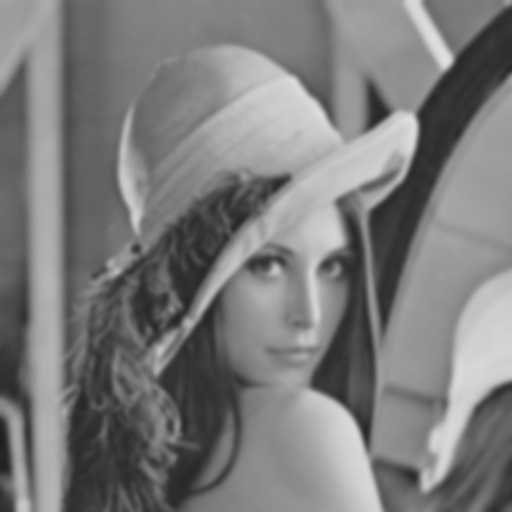
\includegraphics[width=2.5cm]{Lena_scales3.jpg}
				\caption{$\sigma = x$, $N = 7$}
			\end{subfigure}


			\begin{subfigure}[b]{3cm}
				\centering
				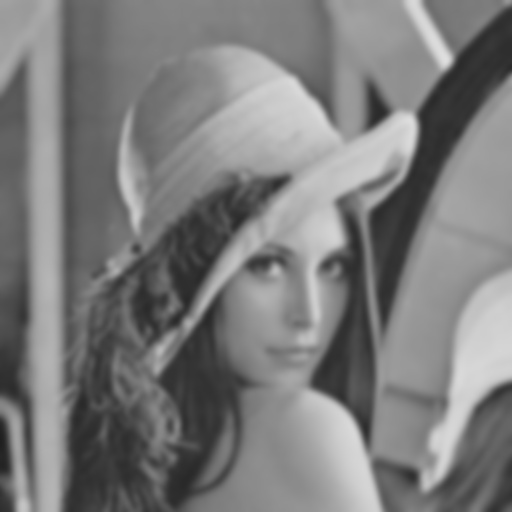
\includegraphics[width=2.5cm]{Lena_scales4.jpg}
				\caption{$\sigma = x$, $N = 9$}
			\end{subfigure}
			~
			\begin{subfigure}[b]{3cm}
				\centering
				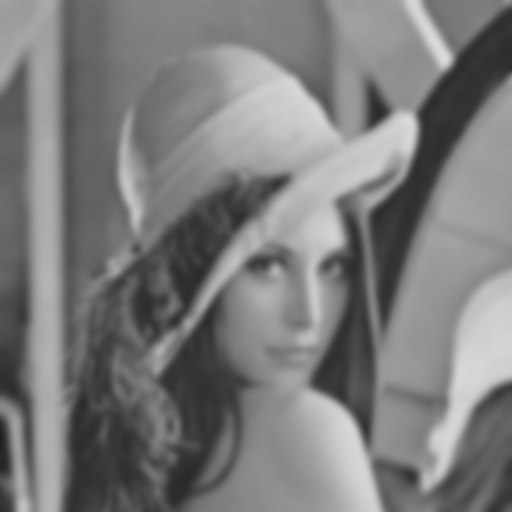
\includegraphics[width=2.5cm]{Lena_scales5.jpg}
				\caption{$\sigma = x$, $N = 11$}
			\end{subfigure}
			~
			\begin{subfigure}[b]{3cm}
				\centering
				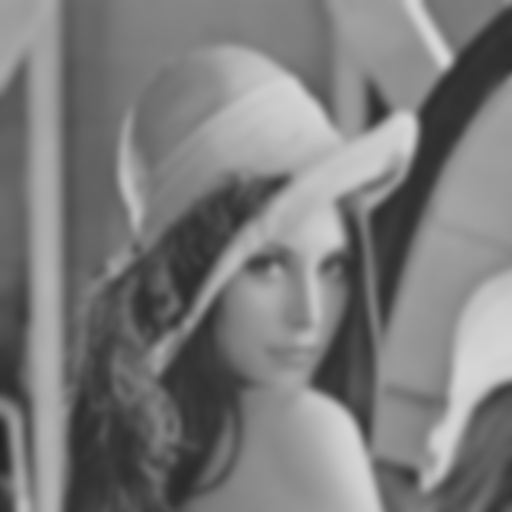
\includegraphics[width=2.5cm]{Lena_scales6.jpg}
				\caption{$\sigma = x$, $N = 13$}
			\end{subfigure}
			\label{lena_scales}
		\end{center}
	\end{figure}
\end{frame}


%---------------------------------------------------------------------------
\begin{frame}
	\frametitle{Przetwarzanie obrazów w przestrzeni skali}

	Po wyznaczeniu reprezentacji skali dla obrazu można przeprowadzić dalsze operacje. W pracy zrealizowano detekcję:	
	\begin{figure}[h]
		\begin{center}
			\begin{subfigure}[b]{5cm}
				\centering
				\includegraphics[width=1cm]{blob.png}
				\caption{plam}
			\end{subfigure}
			~
			\begin{subfigure}[b]{5cm}
				\centering
				\includegraphics[width=1cm]{edge.png}
				\caption{krawędzi}
			\end{subfigure}

			\begin{subfigure}[b]{5cm}
				\centering
				\includegraphics[width=1cm]{corner.png}
				\caption{narożników}
			\end{subfigure}
			~
			\begin{subfigure}[b]{5cm}
				\centering
				\includegraphics[width=1cm]{ridge.png}
				\caption{grani}
			\end{subfigure}
		\end{center}
	\end{figure}
\end{frame}

%---------------------------------------------------------------------------
\begin{frame}
	\frametitle{OpenCL}
	\begin{block}{OpenCL}
		Otwarty, wieloplatformowy standard pozwalający na wykorzystanie procesorów kart graficznych oraz innych urządzeń (w tym wielordzeniowe procesory CPU) w celu wykonywania obliczeń ogólnego przeznaczenia. Wykorzystanie karty graficznej pozwala na zrównoleglenie obliczeń.
	\end{block}

\end{frame}


%---------------------------------------------------------------------------
\begin{frame}
	\frametitle{Użycie OpenCL do zrównoleglenia obliczeń}

	Do implementacji algorytmu z~wykorzystaniem OpenCL konieczne jest:
	\begin{itemize}
		\item Napisanie kodu kerneli - fragmentów kodu wykonywanych na karcie graficznej.
		\item Napisanie kodu wykonywanego na procesorze, który będzie kontrolował część wykonywaną na karcie graficznej. W tym zawiera się przekazanie parametrów do kerneli oraz pobranie wyników.
	\end{itemize}

\end{frame}


%---------------------------------------------------------------------------
\begin{frame}
	\frametitle{Detekcja narożników}



	$$ k = |L_x^2L_{yy}  + L_y^2L_{xx} - 2L_xL_yL_{xy}| $$

	$ k $ - współczynnik krzywizny,

	$ L $ - pochodna wyznaczona z obrazu.
	%Po wyznaczeniu reprezentacji skali obrazu wykonywane są określone operacje matematyczne w~celu detekcji określonych struktur.

	%Poniższy wzór przedstawia sposób detekcji narożników. Wyszukiwane są maksima lokalne wartości $ k $.


\end{frame}
%---------------------------------------------------------------------------
\begin{frame}
	\frametitle{Przykład detekcji}
%\includegraphics[trim=280 200 320 400, clip=true,width=\textwidth]{Operation/input.png}

	\begin{figure}[h]
		\begin{center}

			\begin{subfigure}[b]{3cm}
				\centering
				\includegraphics[trim=280 200 320 400, clip=true,width=\textwidth]{../Operation/input.png}
			\end{subfigure}~
			\begin{subfigure}[b]{3cm}
				\centering
				\includegraphics[trim=280 200 320 400, clip=true,width=\textwidth]{../Operation/blobResult.png}
			\end{subfigure}~
			\begin{subfigure}[b]{3cm}
				\centering
				\includegraphics[trim=280 200 320 400, clip=true,width=\textwidth]{../Operation/edgeResult.png}
			\end{subfigure}

			\begin{subfigure}[b]{3cm}
				\centering
				\includegraphics[trim=280 200 320 400, clip=true,width=\textwidth]{../Operation/null.png}
			\end{subfigure}~
			\begin{subfigure}[b]{3cm}
				\centering
				\includegraphics[trim=280 200 320 400, clip=true,width=\textwidth]{../Operation/cornerResult.png}
			\end{subfigure}~
			\begin{subfigure}[b]{3cm}
				\centering
				\includegraphics[trim=280 200 320 400, clip=true,width=\textwidth]{../Operation/ridgeResult.png}
			\end{subfigure}
			\label{fig:wynik}
		\end{center}
	\end{figure}

\end{frame}
%---------------------------------------------------------------------------
\begin{frame}
	\frametitle{Poprawność rozwiązania}

	Na podstawie porównania z implementacją realizowaną na procesorze CPU stwierdzono, że wykonanie algorytmu na karcie graficznej daje poprawne wyniki.

	Największe rozbieżności są na poziomie 2\%, w~większości przypadków nie przekraczają 1\%.


\end{frame}
%---------------------------------------------------------------------------
\begin{frame}
	\frametitle{Szybkość rozwiązania}

	Z pomiarów czasu obliczeń można zauważyć, że obliczenia na karcie graficznej Nvidia GeForce GTX 670 trwały krócej.

	\begin{center}
		\includegraphics[width=8cm]{../TestySzybkosci/PureAGH.png}
	\end{center}

\end{frame}
%---------------------------------------------------------------------------

\begin{frame}
	\frametitle{}
	\begin{center}
		Dziękuję za uwagę.
	\end{center}
\end{frame}
